%======================================================================
\section{Del lazo abierto al lazo cerrado}\label{sec:cl-intro}
%======================================================================
\noindent Las secciones anteriores responden preguntas sobre \emph{una} decisión: dada una
consulta, ¿qué acción es óptima y con qué garantía? Un controlador predictivo, sin embargo, se
juzga por lo que pasa cuando sus decisiones se aplican una tras otra sobre la planta. Ese
\emph{lazo cerrado} agrega tres efectos que el lazo abierto no ve:
\begin{enumerate}
  \item \textbf{El desajuste del modelo se acumula.} El MPC predice con el ROM (un nodo),
        pero la planta es el HRM (doce nodos). Un error pequeño en cada predicción puede
        sesgar todas las decisiones en la misma dirección.
  \item \textbf{La realimentación corrige.} Cada 0.5~s el MPC vuelve a medir la PCT y
        reoptimiza, así que parte de ese error se corrige solo.
  \item \textbf{Las perturbaciones no previstas} (una falla del ACS, un pronóstico sesgado)
        sólo se pueden evaluar con la planta en el lazo.
\end{enumerate}
\noindent Para cerrar el lazo hace falta la planta. En Simulink, cada consulta del lazo
archivado tarda unos 800~s, y en leo\_acer no hay MATLAB. Por eso el primer paso fue
programar el HRM en Julia, igual que se hizo antes con el ROM. Esta parte presenta ese
trabajo (F1b), las consultas generadas sin Simulink (F4.5), el lazo cerrado determinista
(F5a.1), un Monte Carlo de lazos cerrados (F5a.2), una auditoría de optimalidad de los
solvers y los escenarios extremos (F5a.3). Termina con lo que todo esto implica para la capa
de riesgo.

%======================================================================
\section{El HRM en Julia reproduce Simulink (F1b)}\label{sec:hrm}
%======================================================================
\paragraph{Qué se hizo.} El HRM tiene 50 estados: la potencia, 6 precursores de neutrones
retardados, 6 de calor de decaimiento, las temperaturas de combustible, pared y refrigerante
en 12 nodos axiales y el inventario de refrigerante. Se extrajeron sus ecuaciones bloque a
bloque desde el \code{.slx} y se programaron en \code{julia/SMDFRHRM.jl}, con el mismo
integrador que Simulink (\code{ode1be}: Euler implícito con una iteración de Newton,
$\Delta t=0.5$~s). También se replicó la lógica discreta del DET: el monitor de la banda
[1180, 1220]~K, el planificador que activa la protección, el PI de respaldo y el mapa de la
bomba. La PCT del HRM es el máximo nodal de la temperatura de pared; no usa la regresión
$p_4$ del ROM.

\paragraph{El orden temporal importa.} Al principio la réplica derivaba 0.03~K. La causa
estaba en el momento del paso en que se evalúa cada entrada: en Simulink, las entradas
externas se leen al final del paso ($t_{n+1}$, interpolando y extrapolando), pero la fuga,
que calculan funciones MATLAB controladas por el reloj, se lee al principio ($t_n$). Con esa
convención la réplica coincide con el archivo:

\begin{table}[H]\centering\small
\begin{tabularx}{\linewidth}{@{}Y l@{}}\toprule
Comparación & Error frente al archivo de Simulink\\\midrule
PCT, corrida completa 0--1160~s & $3.2\cdot10^{-6}$~K en 1100--1160~s; $\le8\cdot10^{-6}$~K desde 510~s\\
PCT al final de cada consulta del lazo & $\le5\cdot10^{-6}$~K\\
$T_{e,c}$ del nodo 12 (entrada de la BiLSTM) & $\approx10^{-6}$~K\\
Activación del ACS & 1143.0~s, igual que el archivo\\\bottomrule
\end{tabularx}
\caption{Validación de la réplica del HRM contra la realización archivada.}
\end{table}

\begin{figure}[H]\centering
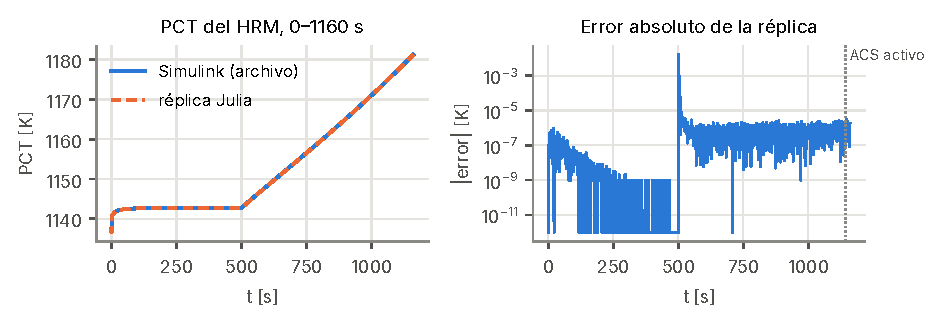
\includegraphics[width=\linewidth]{figures/fig_cl_replica.pdf}
\caption{Réplica del HRM frente a Simulink. El único pico (0.016~K) está en el paso en que
comienza el LOCA (500.5~s) y desaparece en 10~s.}
\end{figure}

\paragraph{Un hallazgo sobre el lazo archivado.} Al repetir las consultas archivadas apareció
un artefacto: en cada consulta, el lazo archivado re-simula el HRM desde $t=0$ con las
corrientes conocidas hasta $t_{k-1}$, y Simulink \emph{extrapola} linealmente la última
entrada: $u(t_k)=2u_{k-1}-u_{k-2}$. En 1160.5~s eso da 113.5~A y una caída ficticia de la PCT
de 34.6~K. El resto de las consultas sufre errores de 0.01--0.04~K por la misma causa. Por eso
la línea base de LJ que se usa abajo es la reconstrucción con la réplica, no la PCT archivada.

\takeaway{La réplica del HRM en Julia reproduce Simulink con un error de $\sim10^{-6}$~K y
corre sin MATLAB. Es la planta de todos los experimentos de lazo cerrado.}

%======================================================================
\section{Consultas sin Simulink y desajuste ROM--HRM (F4.5)}\label{sec:f45}
%======================================================================
Con la réplica del HRM, cada consulta del MPC se construye en Julia, como en el lazo: se
proyecta el estado del HRM sobre el ROM (promedio de los 12 nodos) en $t_q-10$~s y se
calienta el ROM durante 10~s. Las consultas así construidas coinciden con las exportadas de
Simulink: estados con error relativo $\sim10^{-7}$ y predicción de la PCT con error
$7\cdot10^{-7}$~K.

\paragraph{¿Cuánto se equivoca el ROM?} En 41 consultas se resolvió el NLP N3 y su acción se
aplicó al HRM:

\begin{table}[H]\centering\small
\begin{tabularx}{\linewidth}{@{}Y r@{}}\toprule
Indicador (41 consultas, 1160--1180~s) & Valor\\\midrule
Error de la PCT predicha en el instante de la consulta & $-0.06$ a $-0.24$~K (el ROM predice más alto)\\
Error máximo en el horizonte & 0.15--0.25~K\\
Error máximo tras restar el sesgo inicial & $\le0.12$~K\\
Autoridad del actuador (caída de PCT con el caudal máximo) & ROM 2.59~K, HRM 2.33~K\\\bottomrule
\end{tabularx}
\caption{Desajuste entre el ROM y el HRM.}
\end{table}

\noindent El error es pequeño y casi todo es un \textbf{sesgo} constante. El ROM además
sobrestima en un 10\,\% el efecto del actuador. Las dos cosas sugieren un MPC
\emph{offset-free}: medir en cada consulta $d=\mathrm{PCT}_{\rm HRM}-\hat y_{\rm ROM}$ y
seguir $y_{\rm ref}-d$ en lugar de $y_{\rm ref}$.

\paragraph{¿Cambia la decisión?} Para saberlo se resolvió el mismo problema con el HRM
completo como modelo de predicción (N3-HRM: un NLP de 50 estados, 0.5--4~s por consulta), que
hace de oráculo. En 9 consultas la primera acción es idéntica con el ROM, con el ROM más sesgo
y con el oráculo. Medido sobre el HRM, el plan completo del ROM cuesta un 6\,\% (caja
archivada) y un 20\,\% (actuador físico) más que el del oráculo; con la corrección de sesgo,
sólo un 0.3\,\% y un 0.5\,\%.

\takeaway{El ROM basta como modelo de predicción si se corrige su sesgo. Usar el HRM dentro
del MPC no cambia la primera acción y cuesta diez veces más.}

%======================================================================
\section{Lazo cerrado determinista (F5a.1)}\label{sec:f5a1}
%======================================================================
\paragraph{El banco.} \code{julia/ClosedLoop.jl} reproduce la temporización del lazo
archivado. En cada consulta $t_q$: (1) se construye la consulta desde el HRM; (2) el MPC
decide el caudal de los 26 pasos siguientes; (3) se aplica el primero al HRM durante 0.5~s;
(4) se avanza a $t_q+0.5$. A diferencia del lazo archivado, la planta se simula una sola vez
hacia adelante, sin el artefacto de extrapolación. Se comparan N1 (QP con una
linealización), N2 (iteración de tiempo real: un QP linealizado sobre la predicción
desplazada) y N3 (NLP), con y sin corrección de sesgo, y con dos actuadores: la caja
archivada (0--12.86~kg/s, rampa blanda) y el actuador físico (0--5543~kg/s, rampa dura de
5~kg/s por paso).

\begin{table}[H]\centering\small
\begin{tabular}{@{}llrrrr@{}}\toprule
Actuador & Controlador & ISE [K$^2$] & $|e|$ final [K] & Tiempo p99 [s] & Fallas\\\midrule
--- & Sin ACS & 274.2 & 2.92 & --- & ---\\
Archivado & Caudal máximo constante & 42.02 & 0.32 & --- & ---\\
Archivado & LJ archivado (reconstruido) & 46.70 & 0.44 & $\approx800$ & ---\\
Archivado & N1 / N2 / N3 & 41.53 & 0.25 & 0.05 / 0.04 / 0.20 & 0\\
Archivado & N1 / N2 / N3 + sesgo & 41.52 & 0.24 & 0.04 / 0.04 / 0.25 & 0\\
Físico & N1 / N2 / N3 & 24.11--24.12 & 0.05 & 0.06 / 0.04 / 0.24 & 0\\
Físico & N1 / N2 / N3 + sesgo & 23.97 & 0.01 & 0.04 / 0.03 / 0.67 & 0\\\bottomrule
\end{tabular}
\caption{Lazo cerrado sobre la realización archivada, 40 consultas (1160--1179.5~s, la
ventana de LJ). En la ventana de 61 consultas la corrección de sesgo baja el error final de
0.04 a 0.01~K.}
\end{table}

\begin{figure}[H]\centering
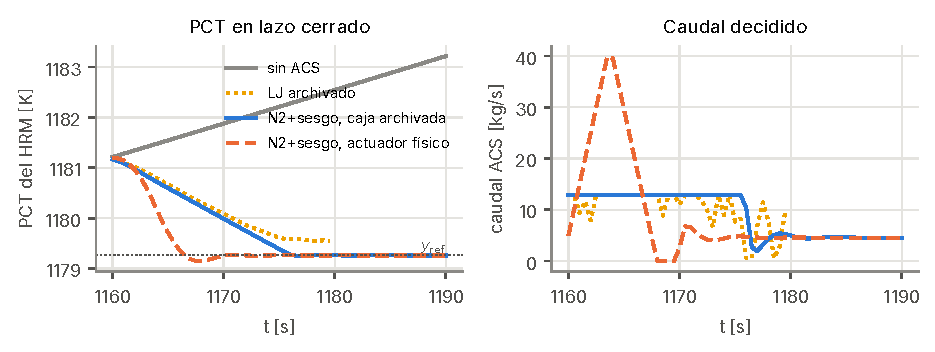
\includegraphics[width=\linewidth]{figures/fig_cl_loop.pdf}
\caption{PCT del HRM y caudal decidido. Con la caja archivada el MPC satura unos 15~s y luego
sigue la referencia; con el actuador físico llega en 6~s.}
\end{figure}

\takeaway{En lazo cerrado, N1, N2 y N3 dan el mismo resultado. El MPC mejora a LJ en un
11\,\% de ISE y tarda $10^4$ veces menos. El actuador físico reduce el ISE a la mitad: pesa
más que la elección del optimizador.}

%======================================================================
\section{Monte Carlo de lazos cerrados (F5a.2)}\label{sec:f5a2}
%======================================================================
\paragraph{Diseño.} Una realización archivada no basta para comparar controladores. El
Monte Carlo sortea la fuga en los rangos del modelo ($A\sim U(0.2,0.4)$, $B\sim U(9,15)$,
$d\sim U(8,10)$~kg/s) y la aplica a todos los controladores (\emph{números aleatorios
comunes}), así que cada comparación es pareada: se resta, realización por realización, el
ISE de la referencia (N3 con sesgo y el mismo actuador). Hay dos familias:
\begin{itemize}
  \item \textbf{Nominal}: sólo cambia la fuga, con pronóstico perfecto.
  \item \textbf{Estresada}: además, perturbaciones que el MPC no conoce: el ACS entrega el
        80--100\,\% del caudal pedido, falla durante 5--15~s, y el pronóstico de fuga tiene
        un error constante de $-0.25$ a $0.05$~kg/s (el sentido del sesgo de la BiLSTM).
\end{itemize}

\begin{table}[H]\centering\small
\begin{tabular}{@{}llrrrr@{}}\toprule
& & \multicolumn{2}{c}{Nominal} & \multicolumn{2}{c}{Estresada}\\\cmidrule(lr){3-4}\cmidrule(l){5-6}
Actuador & Controlador & ISE & $\Delta$ISE & ISE & $\Delta$ISE\\\midrule
--- & Sin ACS & 1958 & --- & 1877 & ---\\
Archivado & Caudal máximo & 878 & +2244\,\% & 198 & +271\,\%\\
Archivado & N1+sesgo, N2+sesgo & 38.74 & $<10^{-4}$\,\% & 54.42 & $<10^{-4}$\,\%\\
Archivado & N2 sin sesgo & 38.88 & +0.38\,\% & 57.46 & +7.0\,\%\\
Archivado & N3+sesgo (ref.) & 38.74 & 0 & 54.42 & 0\\
Físico & N1+sesgo, N2+sesgo & 22.72 & $<10^{-2}$\,\% & 26.84 & $<10^{-3}$\,\%\\
Físico & N2 sin sesgo & 22.99 & +1.2\,\% & 31.75 & +19.5\,\%\\
Físico & N3+sesgo (ref.) & 22.72 & 0 & 26.84 & 0\\\bottomrule
\end{tabular}
\caption{Seis realizaciones (3 por familia), 121 consultas (60~s) cada una, 7260 decisiones
del MPC sin fallas. $\Delta$ISE es la diferencia pareada media contra N3+sesgo con el mismo
actuador. Tiempo p99 por consulta: $\le0.18$~s (QP) y $\le0.71$~s (NLP).}
\end{table}

\takeaway{Con 6 realizaciones, la conclusión de una sola realización se sostiene: N1, N2 y
N3 son indistinguibles cuando tienen corrección de sesgo. La corrección vale más cuanto más
perturbada está la planta (de +0.4\,\% a +19\,\% de ISE sin ella). El actuador físico
reduce el ISE en un 41--51\,\%.}

%======================================================================
\section{¿Los solvers resuelven a optimalidad?}\label{sec:auditoria}
%======================================================================
El conteo de fallas anterior trata como éxito la salida \emph{aceptable} de Ipopt
(\code{ALMOST\_LOCALLY\_SOLVED}). Para saber si eso esconde algo, a lo largo de un lazo
N3+sesgo (726 consultas: la realización archivada y dos del Monte Carlo, con los dos
actuadores) cada consulta se resolvió de cinco maneras, y todas las soluciones se evaluaron
con el mismo costo P0 sobre el ROM (\code{julia/f5a\_optimality\_audit.jl}).

\begin{table}[H]\centering\footnotesize\setlength{\tabcolsep}{4pt}
\begin{tabularx}{\linewidth}{@{}l Y r r@{}}\toprule
Solver & Estado de terminación (726 consultas) & Brecha [K$^2$] (mediana / máx.) & $|\Delta\mdot_0|$ máx.\ [kg/s]\\\midrule
N1 (QP) & óptimo: 726 & $10^{-6}$ / 0.0097 & 0.11\\
N2 (QP) & óptimo: 726 & $5\cdot10^{-12}$ / 0.0022 & 0.01\\
N3 en el lazo & óptimo local: 160; aceptable: 566 & $2\cdot10^{-14}$ / $3\cdot10^{-8}$ & ---\\
N3 sin salida aceptable & igual, más 7 por límite de iteraciones & idéntica & $2\cdot10^{-7}$\\
N3 con arranque en frío & igual & 0 / $4\cdot10^{-8}$ & 0.0015\\\bottomrule
\end{tabularx}
\caption{Auditoría de optimalidad. La brecha de costo se mide contra el mejor N3 de cada
consulta. Estados: óptimo = \code{OPTIMAL} (Clarabel); óptimo local = \code{LOCALLY\_SOLVED}
y aceptable = \code{ALMOST\_LOCALLY\_SOLVED} (Ipopt).}
\end{table}

\begin{itemize}
  \item N1 y N2 resuelven su QP convexo al óptimo global. Ese óptimo es el del modelo
        linealizado; medido sobre P0, la pérdida es $\le0.01$~K$^2$ y sólo aparece en las
        primeras consultas, donde el costo vale 15--46~K$^2$.
  \item N3 termina en la salida aceptable en el 78\,\% de las consultas porque, en régimen,
        el costo óptimo es $\approx3\cdot10^{-12}$~K$^2$: el seguimiento es perfecto y la
        tolerancia de $10^{-10}$ queda bajo el ruido numérico. Sin la salida aceptable, o
        desde un arranque en frío, llega al mismo punto.
\end{itemize}

\takeaway{Todas las decisiones del lazo son óptimas para su problema: global en N1 y N2
(QP convexos) y local reproducible en N3. La optimalidad global de N3 sólo está certificada
en las dos consultas de la sección~\ref{sec:certificacion}.}

%======================================================================
\section{Escenarios extremos: ¿dónde está el riesgo? (F5a.3)}\label{sec:extremos}
%======================================================================
\paragraph{Por qué hacen falta.} En las familias nominal y estresada ningún controlador pasó
de 1185~K, ni siquiera sin ACS. Una capa de riesgo sobre un límite que nunca se acerca
estaría siempre inactiva y daría lo mismo que el MPC determinista. Antes de diseñarla hay que
saber en qué escenarios la seguridad está realmente en juego.

\paragraph{El límite que importa es 1220~K.} El monitor del DET clasifica la PCT en tres
estados: bajo 1180~K, en la banda [1180, 1220]~K y sobre 1220~K. En Simulink, el tercer
estado \emph{detiene la simulación}: es el estado final del árbol de eventos. Por eso las
corridas de esta sección terminan cuando la PCT cruza 1220~K, y ese cruce se cuenta como el
evento de falla. El límite $U_y=1244$~K de la función de costo queda más allá.

\paragraph{Barrido de severidad.} Primero se simuló sólo el HRM, con la lógica del DET, para
fugas cada vez más severas:

\begin{table}[H]\centering\small
\begin{tabularx}{\linewidth}{@{}Y r r r l@{}}\toprule
Fuga ($d$, $A$, $B$) & Activación & Fuga & PCT máx.\ (PI) & Sin ACS: 1180 $\to$ 1220~K\\\midrule
10, 0.28, 10 ($\approx$ archivada) & 1134~s & 4.7~kg/s & 1189~K & 1134 $\to$ 1649~s\\
15, 0.20, 10 & 823~s & 9.7~kg/s & 1198~K & 822 $\to$ 1065~s\\
20, 0.20, 15 & 724~s & 14.3~kg/s & 1206~K & 723 $\to$ 886~s\\
20, 0.10, 15 & 690~s & 17.2~kg/s & 1211~K & 688 $\to$ 823~s\\
30, 0.10, 10 & 629~s & 25.1~kg/s & --- & inventario agotado en 820~s\\\bottomrule
\end{tabularx}
\caption{Severidad de la fuga, sin MPC. ``Fuga'' es su magnitud en la activación del ACS y
``PI'' el controlador de respaldo del DET.}
\end{table}

\begin{itemize}
  \item Sin ACS, la PCT llega a 1220~K en 130--240~s con fugas severas, y en unos 500~s con
        la fuga archivada.
  \item El PI del DET contiene todas las fugas, con caudales de 370--530~kg/s, pero tarda:
        su integrador necesita unos 150~s para alcanzar el umbral de la bomba.
  \item Con fugas de 10--17~kg/s, la caja archivada (12.86~kg/s) ya no compensa la fuga.
\end{itemize}

\paragraph{La familia extrema.} Combina las dos fuentes de riesgo propuestas: (a)
escenarios más severos y (c) la caja archivada, cuya capacidad queda por debajo de la fuga.
Cada realización sortea:
\begin{itemize}
  \item fuga $d\sim U(15,25)$~kg/s, $A\sim U(0.1,0.2)$, $B\sim U(10,15)$;
  \item el inicio del MPC entre 0 y 17~s después de la activación (fase aguda);
  \item un ACS que entrega el 60--90\,\% de lo pedido y falla durante 30--90~s;
  \item un error del pronóstico de fuga de $-0.5$ a $0.1$~kg/s.
\end{itemize}
Se comparan, durante 240~s: sin ACS, caudal máximo constante, el PI del DET y N2 con y sin
sesgo con los dos actuadores. N1 y N3 se omiten porque coinciden con N2, y la referencia
pareada pasa a ser N2+sesgo.

\paragraph{Resultados} (14 realizaciones, \code{results/f5a2\_monte\_carlo/runs\_extreme.csv}).

\begin{table}[H]\centering\footnotesize\setlength{\tabcolsep}{4pt}
\begin{tabularx}{\linewidth}{@{}l Y r r r r@{}}\toprule
Actuador & Controlador & Llega a 1220~K & Tiempo hasta 1220~K & PCT máx.\ si no llega & Masa inyectada\\\midrule
--- & Sin ACS & 14/14 & 113--181~s (media 140) & --- & 0\\
Archivado & Caudal máximo, N2, N2+sesgo & 9/14 & 155--251~s (media 191) & 1206--1219~K & 470--2070~kg\\
--- & PI del DET & 0/14 & --- & 1204--1216~K & 5300--6360~kg\\
Físico & N2 / N2+sesgo & 0/14 & --- & 1189--1207~K & 3260--5170~kg\\\bottomrule
\end{tabularx}
\caption{Familia extrema. Los tiempos se cuentan desde la activación del ACS. Las tres
variantes con la caja archivada dan resultados idénticos en las 14 realizaciones. Tiempo p99
por consulta de N2: $\le0.19$~s, sin fallas del solver.}
\end{table}

\begin{figure}[H]\centering
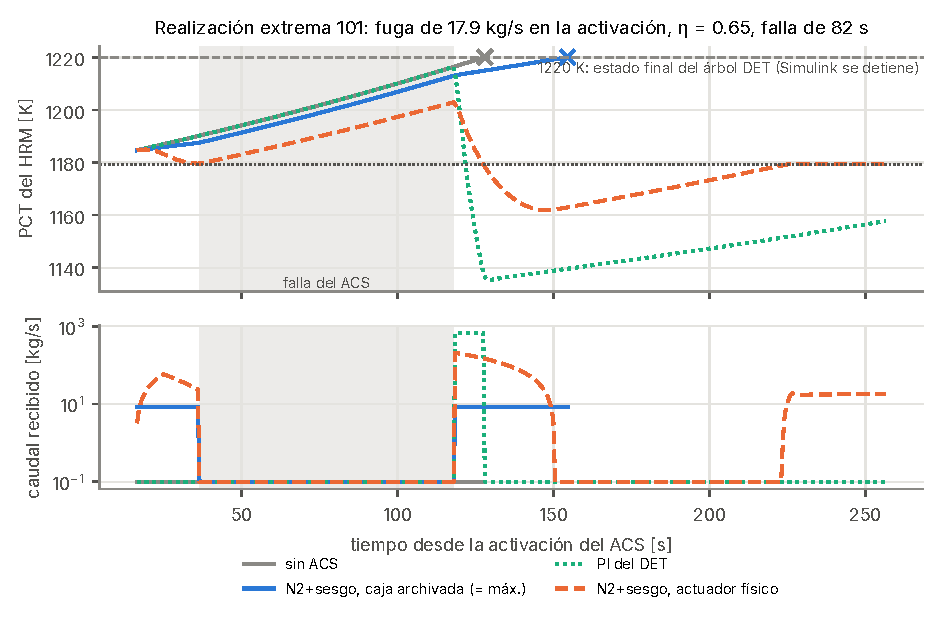
\includegraphics[width=\linewidth]{figures/fig_cl_extreme.pdf}
\caption{Una realización extrema. Sin ACS, la PCT llega a 1220~K a los 128~s (cruz gris). Con
la caja archivada, el MPC satura en todo momento (igual que el caudal máximo) y sólo retrasa
el cruce hasta los 155~s (cruz azul). El PI del DET reacciona tarde pero con fuerza (hasta
670~kg/s) y enfría hasta 1135~K. N2 con el actuador físico deja subir la PCT durante la falla
hasta 1203~K y vuelve a la referencia sin sobreenfriar.}
\end{figure}

\begin{figure}[H]\centering
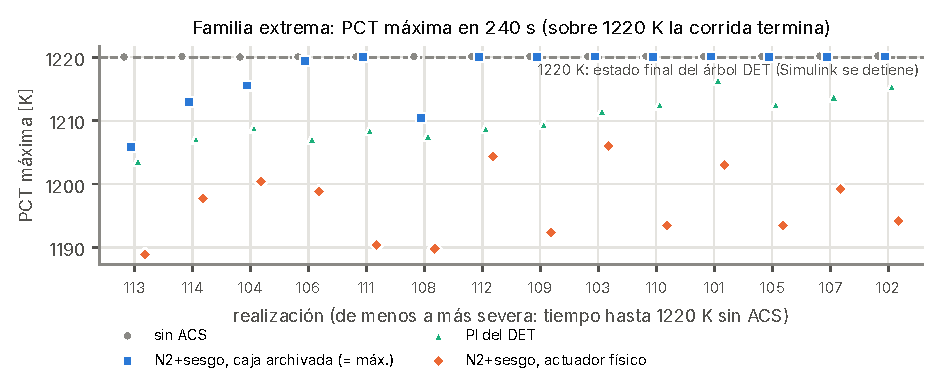
\includegraphics[width=\linewidth]{figures/fig_cl_extreme_max.pdf}
\caption{PCT máxima por realización. Los puntos sobre la línea de 1220~K son corridas que
alcanzaron el estado final del DET.}
\end{figure}

\paragraph{Cómo leer estos resultados.}
\begin{enumerate}
  \item \textbf{Con la caja archivada, el optimizador no importa.} En las 14 realizaciones
        el MPC decide el caudal máximo en cada consulta: la fuga supera la capacidad. N2, N2
        con sesgo y el caudal máximo constante dan exactamente la misma trayectoria, y 9 de
        14 llegan al estado final del DET, en promedio unos 60~s después de lo que llegarían sin ACS. Una
        capa de riesgo tampoco cambiaría nada: no hay decisión que tomar, sólo capacidad.
  \item \textbf{Con el actuador físico, el límite queda lejos.} Ninguna realización pasa de
        1207~K, aun con fallas de hasta 90~s y un ACS al 60\,\%. El margen mínimo es de 13~K.
        El MPC inyecta un 25\,\% menos de masa que el PI del DET y no sobreenfría.
  \item \textbf{La corrección de sesgo pierde precisión con fallas del ACS.} El calentamiento
        del ROM usa los caudales \emph{pedidos}, así que el gemelo no sabe que el ACS falló.
        La corrección de sesgo absorbe esa diferencia, pero como un sesgo constante: en esta
        familia, N2 con y sin sesgo no se distinguen ($\Delta$ISE $=-16\,000\pm21\,000$~K$^2$).
        Si el caudal real del ACS se mide, el gemelo debería usarlo.
\end{enumerate}

\takeaway{El riesgo de cruzar 1220~K existe en esta familia, pero en los dos actuadores
probados no depende de la decisión: con la caja archivada nada lo evita, y con el actuador
físico nunca ocurre. La capa de riesgo sólo puede aportar en el régimen intermedio, con una
capacidad comparable a la fuga y fallas largas del ACS. Ahí conviene mantener un margen bajo
la referencia ante una falla posible. Ése es el banco de pruebas que debe tener F5b.}

%======================================================================
\section{Lo que esto implica para la capa de riesgo}\label{sec:implicancias}
%======================================================================
\begin{enumerate}
  \item \textbf{Dónde montarla: sobre N2.} N1, N2 y N3 dan las mismas decisiones en lazo
        cerrado. N2 es un QP de $\sim30$~ms, así que admite escenarios y restricciones de
        riesgo sin salir del tiempo real.
  \item \textbf{Qué riesgo: cruzar 1220~K}, el estado final del DET, en escenarios con
        capacidad del actuador comparable a la fuga y fallas largas del ACS. El primer paso es
        un barrido de capacidad (15--50~kg/s con rampa dura) para ubicar ese régimen.
  \item \textbf{Corrección de la PCT: se mantiene $p_4$ con sesgo.} En la arquitectura de
        caja gris del gemelo, la parte de caja negra que corrige la PCT del ROM es el
        polinomio $p_4$, no la BiLSTM. Tras la corrección de sesgo, el desajuste ROM--HRM es
        $\le0.12$~K. Reentrenar una red sobre la diferencia de PCT entre el HRM y el modelo de
        caja blanca no se justifica con un residuo de ese tamaño.
  \item \textbf{Pronóstico de fuga: la BiLSTM, con su error modelado.} La réplica del HRM le
        entrega las mismas entradas que Simulink (fuga y $T_{e,c}$ del nodo 12), así que no hace
        falta ajustarla para usarla con la réplica. Sí haría falta en la familia extrema, que
        queda fuera de su rango de entrenamiento ($A\sim U(0.2,0.4)$, $d\sim U(8,10)$). El
        orden propuesto es: un modelo de error calibrado sobre sus residuos, un ajuste
        paramétrico de la ley de Park como alternativa sin red y, sólo si las decisiones de
        riesgo resultan sensibles al pronóstico, un ajuste fino con datos de la réplica.
  \item \textbf{Cómo evaluarla:} en forma pareada contra N2+sesgo, midiendo la frecuencia del
        cruce de 1220~K, la PCT máxima, el margen y el costo de la prudencia (masa inyectada y
        error de seguimiento).
\end{enumerate}


